\documentclass{beamer}

\usepackage[utf8]{inputenc}
\usecolortheme{beaver}
\usepackage{caption}
\usepackage{subcaption}
\usepackage{mathtools}
\usepackage{todonotes}
\usepackage{amsmath}
\usepackage{bm}
\usepackage{listings}
\usepackage{ragged2e}
\usepackage{titlecaps}
\usepackage{fancyvrb}

\def\ci{\perp\!\!\!\!\!\perp}

\newtheorem{proposition}{Proposition}
\Addlcwords{for a is but and with of in as the etc on to if}

\setbeamertemplate{section in toc}{\inserttocsectionnumber.~\inserttocsection}
\usetheme{Boadilla}
\makeatletter
\setbeamertemplate{footline}{%
    \leavevmode%
    \hbox{%
        \begin{beamercolorbox}[wd=.3\paperwidth,ht=2.25ex,dp=1ex,center]{author in head/foot}%
            \usebeamerfont{author in head/foot}\insertshortauthor\expandafter\beamer@ifempty\expandafter{\beamer@shortinstitute}{}{~~(\insertshortinstitute)}
        \end{beamercolorbox}%
        \begin{beamercolorbox}[wd=.55\paperwidth,ht=2.25ex,dp=1ex,center]{title in head/foot}%
            \usebeamerfont{title in head/foot}\insertshorttitle
        \end{beamercolorbox}%
        \begin{beamercolorbox}[wd=.15\paperwidth,ht=2.25ex,dp=1ex,right]{date in head/foot}%
            \usebeamerfont{date in head/foot}\insertshortdate{}\hspace*{2em}
            \insertframenumber{} / \inserttotalframenumber\hspace*{2ex} 
        \end{beamercolorbox}}%
        \vskip0pt%
    }
\makeatother

\begin{document}

\title[]{Canonical Correlation Based Mixed Data Conditional Independence Testing: Empirical Analysis}
\author{}
\date{}

\maketitle

\begin{frame}{CI Tests}
	\begin{enumerate}
		\item Mutual Information based test (MI-CG) \footnotemark
			\begin{itemize}
				\item Used as baseline.
				\item Equivalent to chi-squared test for discrete variables.
			\end{itemize}
		\item Likelihood Ratio Test (MXM) \footnotemark
			\begin{itemize}
				\item Compares the likelihood of $ X \sim \bm{Z} $ and $ X \sim \bm{Z} + Y $.
				\item Regression method chosen based on data type.
			\end{itemize}
		\item Hotelling's $T^2$ test on residuals. \footnotemark
		\item Pillai's Trace: A canonical correlation based test.
	\end{enumerate}

\footnotetext[1]{Scutari, Marco, Maintainer Marco Scutari, and Hiton-PC MMPC. "Package ‘bnlearn’." Bayesian network structure learning, parameter learning and inference}
\footnotetext[2]{Michail Tsagris, Giorgos Borboudakis, Vincenzo Lagani, and Ioannis Tsamardinos. Constraint-based causal discovery with mixed data.}
\footnotetext[3]{Ankan, Ankur, and Johannes Textor. A simple unified approach to testing high-dimensional conditional independences for categorical and ordinal data}

\end{frame}

\begin{frame}{Hotelling's $ T^2 $ on Residuals}

Given two residual matrices, $ R_{\mathbf{x}}: \mathbf{x} \sim \mathbf{z} $ and $ R_{\mathbf{y}}: \mathbf{y} \sim \mathbf{z} $, the $ T^2 $ test statistic is given as:

\begin{equation}
	Q(\mathbf{x}, \mathbf{y}) = \frac{1}{n} \left( d \times \hat{\Sigma}_d \times d^T \right)
\end{equation}
where,

\begin{eqnarray*}
d &  =  & (R_{\mathbb{I}(\mathbf{x}=1)} \cdot R_{\mathbb{I}(\mathbf{y}=1)}, \, \ldots \ ,
R_{\mathbb{I}(\mathbf{x}=k-1)} R_{\mathbb{I}(\mathbf{y}=1)}, \, \ldots \, ,
\\
 &  & R_{\mathbb{I}(\mathbf{x}=1)} \cdot R_{\mathbb{I}(\mathbf{y}=r-1)}, \, \ldots \ ,
R_{\mathbb{I}(\mathbf{x}=k-1)} R_{\mathbb{I}(\mathbf{y}=r-1)}
) \\
\hat{\Sigma}_d & = &\textrm{cov}(d)
\end{eqnarray*}

% \begin{equation}
% 	\begin{split}
% 		d &= (R_{\mathbb{I}(\mathbf{x}=1)} \cdot R_{(\mathbf{y}=1)}, \, \ldots \ , R_{\mathbb{I}(\mathbf{x}=C_x)} \cdot R_{(\mathbf{y}=C_y)} ) \\
% 		\hat{\Sigma}_d &= \textrm{cov}(d)
% 	\end{split}
% \end{equation}


Under null, $ Q $ is asymptotically $ \chi^2 (\mid d \mid) $ distributed.

\end{frame}

\begin{frame}{Pillai's Trace on Residuals}
Given two residual matrices, $ R_{\mathbf{x}}: \mathbf{x} \sim \mathbf{z} $ and $ R_{\mathbf{y}}: \mathbf{y} \sim \mathbf{z} $, Pillai's Trace is given as:

\begin{equation}
	\textit{V}(R_\mathbf{x}, R_\mathbf{y}) = \sum_{\rho \in \bm{\rho}(R_\mathbf{x}, R_\mathbf{y})} \rho^2
\end{equation}
where, $ \bm{\rho}({R_\mathbf{x}, R_\mathbf{y}}) $  is the canonical correlation between $ R_\mathbf{x} $ and $ R_\mathbf{y} $.

\vspace{1em}

No exact asymptotic distribution of $ V $ is known, but p-values can be computed using F-approximation. \footnotemark

\footnotetext[4]{Muller, Keith E., and Bercedis L. Peterson. "Practical methods for computing power in testing the multivariate general linear hypothesis."}
\end{frame}

\begin{frame}{Simulating Mixed Data}
	Given a node $ Y $ with parents $ Pa_Y $, $ Y $ is simulated as follows:
	\begin{enumerate}
		\item Categorical variables in $ Pa_Y $ are dummy encoded. Ordinal variables are treated as continuous.
		\item \begin{itemize}
			\item If $ Y $ is continuous, simple linear regression.
			% \item If $ Y $ is continuous, $ Y = \mathbf{B} Pa_Y + \epsilon $
			\item If $ Y $ is categorical, multinomial logistic regression.
			% \item If $ Y $ is categorical, $ Y \sim \lambda(\mathbf{B} Pa_Y + \epsilon) $, where $ \lambda(x) = \frac{e^x}{1+e^x} $.
			\item If $ Y $ is ordinal, proportional odds logistic regression.
			% \item If $ Y $ is ordinal, using proportional odds logistic regression. $ Y \sim \lambda(A + \mathbf{B} Pa_Y + \epsilon) $.
		\end{itemize}
	\end{enumerate}
\todo[inline]{Add more details here}
\end{frame}

\begin{frame}{Calibration: Data Generation}
	We use the following DAG:
\begin{center}
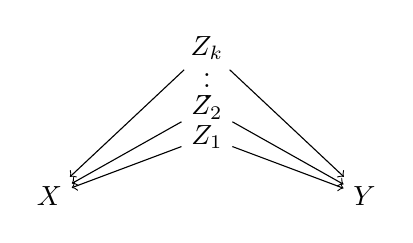
\begin{tikzpicture}[yscale=.75]
	\node (x) at (-1,1) {$X$};
	\node (y) at (3,1) {$Y$};
	\node (z) at (1,2) {$Z_1$};
	\node (z2) at (1, 2.5) {$Z_2$};
	\node (dots) at (1, 3) {$ \vdots $};
	\node (zk) at (1, 3.5) {$ Z_k $};
	\draw [->] (z) -- (y);
	\draw [->] (z) -- (x);
	\draw [->] (z2) -- (x);
	\draw [->] (z2) -- (y);
	\draw [->] (zk) -- (x);
	\draw [->] (zk) -- (y);
\end{tikzpicture}
\end{center}

\end{frame}

\begin{frame}{Calibration: Mixed Data}
	\begin{figure}[t]
		\centering
		\includegraphics{../../2023-canonical-cor/code/plots/calibration_mixed.pdf}
	\end{figure}
\end{frame}

\begin{frame}{Calibration: Discrete Data}
	\begin{figure}[t]
		\centering
		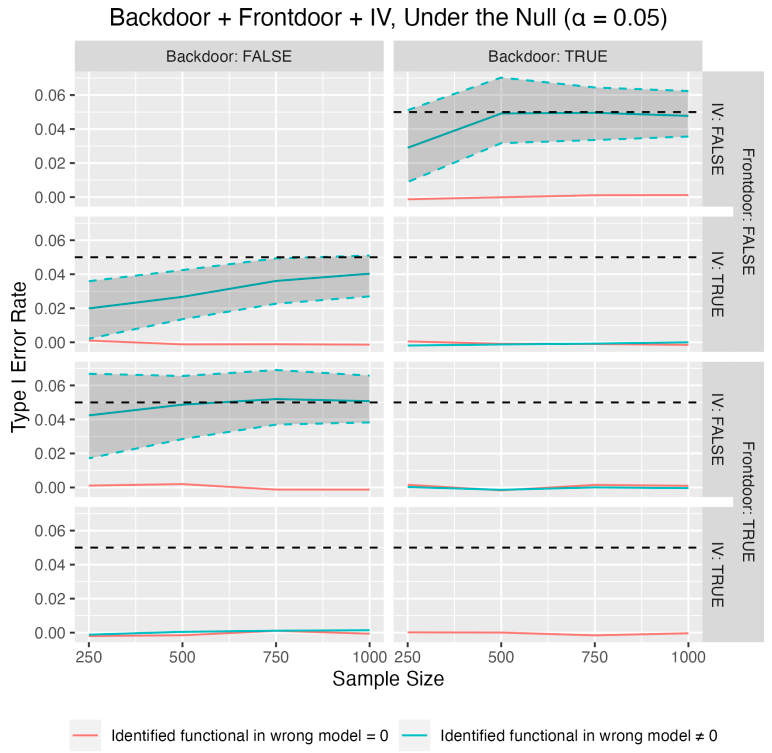
\includegraphics{../../2023-canonical-cor/code/plots/calibration.pdf}
	\end{figure}
\end{frame}

\begin{frame}{Accuracy: Data Generation}
	We use the DAG:

\begin{center}
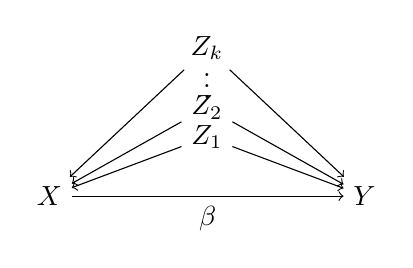
\begin{tikzpicture}[yscale=.75]
	\node (x) at (-1,0) {$X$};
	\node (y) at (3,0) {$Y$};
	\node (z) at (1,1) {$Z_1$};
	\node (z2) at (1, 1.5) {$Z_2$};
	\node  at (1, 2) {$ \vdots $};
	\node (zk) at (1, 2.5) {$Z_k$};
	\draw [->] (x) edge node [midway, below] {$\beta$} (y);
	\draw [->] (z) -- (y);
	\draw [->] (z) -- (x);
	\draw [->] (z2) -- (y);
	\draw [->] (z2) -- (x);
	\draw [->] (zk) -- (y);
	\draw [->] (zk) -- (x);
\end{tikzpicture}
\end{center}
\end{frame}

\begin{frame}{Accuracy: Mixed Data}
	\begin{figure}[t]
		\centering
		\includegraphics{../../2023-canonical-cor/code/plots/accuracy_mixed.pdf}
	\end{figure}
\end{frame}

\begin{frame}{Accuracy: Categorical Data}
	\begin{figure}[t]
		\centering
		\includegraphics{../../2023-canonical-cor/code/plots/accuracy_cat.pdf}
	\end{figure}
\end{frame}


\begin{frame}{Structure Learning: Data Generation}
	DAG generation mechanism.
\end{frame}

\begin{frame}{Structure Learning: Mixed Data}
\end{frame}

\begin{frame}{Structure Learning: Categorical Data}
\end{frame}

\begin{frame}{Conclusion}
	\begin{itemize}
		\item Pillai's Trace is better calibrated especially in high-dimensional scenarios.
	\end{itemize}
\end{frame}

\end{document}
